\documentclass[twoside,onecolumn,12pt,letterpaper]{article}
\usepackage{setspace}
%\doublespacing

\usepackage[utf8]{inputenc}
\usepackage{amsmath}
\usepackage{amsfonts}
\usepackage{amssymb}
\usepackage{graphicx}
\usepackage{mathtools}
\usepackage[left=2cm,right=2cm,top=2cm,bottom=2cm]{geometry}
\usepackage{placeins}

\allowdisplaybreaks[1] %breaks multipage equations in align environment
\setlength{\abovedisplayskip}{12pt} %spacing above equations
\setlength{\belowdisplayskip}{12pt} %spacing below equations

\usepackage{hyperref} % For hyperlinks in the PDF
\usepackage{enumitem}
\usepackage{tikz}
\usetikzlibrary{arrows, positioning, automata}
\usepackage{subcaption}
\usepackage{array,multirow}

\usepackage{natbib}   
\bibliographystyle{plainnat}
%\bibliographystyle{apalike} 

\newtheorem{example}{EXAMPLE}

\usepackage{abstract} % Allows abstract customization
\renewcommand{\abstractnamefont}{\normalfont\bfseries} % Set the "Abstract" text to bold
\renewcommand{\abstracttextfont}{\normalfont\small\itshape} % Set the abstract itself to small italic text

\newbox\flinebox 
\newbox\slinebox
\newbox\mlinebox
\def\duplines{\setlength\parindent{0pt}
  \setbox\flinebox\lastbox
  \ifvoid\flinebox\relax
  \else
  \setbox\slinebox\hbox{\copy\flinebox}
  \setbox\mlinebox\hbox{\copy\flinebox}
  \unskip\unpenalty
  {\duplines}
  \box\flinebox\vspace*{-3.3ex}
  \box\mlinebox\vspace*{-3.3ex}
  \box\slinebox \fi
}

\newcommand\BlurText[1]{%
  \vbox{#1\par\duplines}}
  
\usepackage{textcomp}
%\sffamily\textregistered\textcopyright
\usepackage{fancyhdr} % Headers and footers
\pagestyle{fancy} % All pages have headers and footers
\fancyhead{} % Blank out the default header
\fancyfoot{} % Blank out the default footer
\fancyfoot[C]{Copyright \textsuperscript{\copyright} 2018, Sanchit Singh. All rights reserved} % Custom header text
\fancyfoot[RO,LE]{\thepage} % Custom footer text

\title{\bfseries Mass Customization: Using Commonality of Sub-assemblies To Reduce Assemble To Order (ATO) Cost} % Article title

\author{
\textsc{Sanchit Singh \thanks{\href{mailto:sanchit@vt.edu}{sanchit@vt.edu}}}\\
\normalsize Grado Department of Industrial and Systems Engineering, \\
\normalsize Virginia Polytechnic Institute and State University \\
}

\date{} % Leave empty to omit a date

\begin{document}
\maketitle
\section{Introduction\label{sec:introduction}}

Today’s highly competitive global market is redefining the way that many companies do business. With significantly shortened product life cycles, manufacturers have found that they can no longer capture market share and gain higher profits by producing large volumes of a standard product for a mass market (\citet{qiao2002general}, \citet{kumar2007scalable}, \citet{qu2011two}). Consequently, companies are faced with the challenge of providing as much variety as possible for the market without having to constantly alter manufacturing system. Such a manufacturing mode is called mass customization (MC), which aims at meeting customers’ diverse requirements without a corresponding increase in cost and lead time via economy of scope (\citet{jiao1998design}). Under the MC environment, many operational benefits such as shorter lead times and lower costs can be derived (\citet{park2008toward}, \citet{zhang2008simultaneous}).

Among many approaches that set us closer to achieving MC, `Platform Product Design' (PPD) constitutes an advanced approach to agile product development (\citet{wheelwright1992revolutionizing}, \citet{meyer1997power}, \citet{robertson1998planning}). It not only aims at creating necessary product variety for competitive success in the marketplace (\citet{salvador2002mass}), but also dramatically controls and often reduces both the production cost and time to market to a competitive level. Leading manufacturers, such as Black and Decker and HP have applied some PPD strategies and techniques to rationalize their product lines (\citet{meyer1997power}). Volkswagen used platform architecture strategy and reduced development and production costs (\citet{wilhelm1997platform}). As a result, they have been able to increase the scope/variety of end-products while reducing the variety of the constituent components and raw materials. \citet{krishnan2001product}, \citet{simpson2004product}, \citet{jose2005modular}, and more recently, \citet{allada2006product} have provided a review of various aspects of product platform development methodologies. \citet{allada2006product} classify research on PPD in two streams: (1) that belongs to the use of qualitative approach (\citet{martin1997design}, \citet{kota2000metric}), and (2) that belongs to the use of quantitative approach with focus on the engineering and design aspects of the products. The research in the quantitative approach can be further divided into: research on scalable (parametric) platforms (\citet{simpson2001balancing}, \citet{hernandez2003platform}), module-based or configuration-based platform formations (\citet{fujita1999product}, \citet{ben2009solving}), and a combination of both module-based and scalable platforms (\citet{fujita2004pro}).

\citet{ben2009solving} describe a platform to be a set of shared components among multiple products. A product of a product family is produced using a particular platform by adding or removing some of the components that are assembled using the particular platform. They propose multiple platforms for the production of a given product family with the aim of minimizing the production cost for mass assembly plus the cost for adding/removing components from the platforms, while considering the individual demand and structure of each product type. 

The work by \citet{ben2009solving} has made an important contribution in the development of theory of products' platform(s) for achieving MC; however, it has the following shortcomings: (1) The constituent elements in a product's ``Bill of materials" (BOM) are treated as components rather than sub-assemblies, which among other things poses a confusing picture of physical assembly of parts that remain inconsistent across products. (2) The resultant platform(s) after optimization might not turn out to be feasible engineering-wise, as they do not incorporate necessary rules and guidelines either a priori or post-optimization. Perhaps, this was done for the sake of simplicity. 

\citet{zhang2010simultaneous} list some cost-effective strategies for PPD - commonality (components are standardized, and then, shared as far as possible without compromising the variety of the end-products entering the market), modularity (standardized modular options are selected, and then, configured according to specific market and business needs), postponement or delayed product differentiation (in which product structures are arranged so that early proliferation of part variety is avoided and variation is allowed and enabled as late as possible in the manufacturing process; see \citet{lee1997modelling}) and scalability (‘serialization and ranging’ of product parameters that have to be changeable; see \citet{simpson2001product}). In our work, we focus on effectively using the concept of commonality. The positive impacts of commonality have been widely demonstrated in relevant studies. For example, high commonality results in simplified planning and scheduling (\citet{berry1992product}), lower setup and holding costs (\citet{collier1981measurement}), lower safety stock (\citet{dogramaci1979design}, \citet{baker1985safety}), reduction of vendor lead time uncertainty (\citet{benton1990vendor}) and order-quantity economies (\citet{gerchak1989component}).

\citet{collier1981measurement} uses regression analysis to relate the performance of MRP system to the degree of commonality index (that measures the commonality of certain sub-assemblies and components across products). It studies the impact of the degree of commonality among component parts to various dependent variables such as total cost, work center load, and delivery performance under three different lot-size models, lot-for-lot (LFL), least total cost (LTC), and economic order quantity (EOQ) over a six week planning horizon. In this paper, we build on this concept and consider the commonality that exists in the assembly hierarchy for products defined by their BOM. Unlike in this study and in the literature that assume a simplistic  form of commonality among products, we broaden the scope by considering commonality of sub-assemblies across products from the viewpoint of reducing overall production cost. 

\textbf{Problem Statement:} We assume an assembly job-shop configuration, wherein different assemblies (products) or sub-assemblies are put together in-house following products' BOM (even though the timing aspect of production is not considered here). Each contiguous assembly operation incurs a setup time and unit production/assembly cost. The sub-assemblies can either be stocked up as inventory after their production/assembly (Stage 1) or assembled from its constituent sub-assemblies as and when the products' demands arise under the stochastic setting (Stage 2). Every unit of sub-assembly assembled during Stage 1, if not utilized incurs unit inventory cost. This feature takes significance only when production is done under a stochastic setting for products' demand. Under the presence of common sub-assemblies across products, for the objective of minimizing the total cost of production, setup and losses due to excessive inventory, some of the commonly used methodologies such as ``Assemble to order" (ATO), ``Make to stock" (MTS) and ``Assemble to Order" (ATO) are evaluated. We also propose a new methodology that is very flexible and performs better than those mentioned above. It is also supposed to deliver satisfactorily results when the timing aspect of production is to be considered where the objective or the constraints also include lead time of orders' fulfillment. 

We make the following assumptions:
\begin{enumerate} [noitemsep, topsep=6pt]
\item Each sub-assembly is prepared from one or more other sub-assemblies and/or base components in-house. This aspect and related cost of assembly operation remains independent of which product is formed. It thus follows naturally that no sub-assembly can occur in the sub-tree of its own when it's ``Bill of Materials" (BOM) is expanded all the way down to terminal sub-assemblies and/or base components.
\item Each contiguous assembly operation for a sub-assembly incurs a fixed sub-assembly dependent setup cost independent of units of sub-assemblies put together. There is also a sub-assembly dependent unit assembly cost. 
\end{enumerate}

Next, we describe two fundamental methods used for in-house production of sub-assemblies and products. We explain their implicit use in commonly used production philosophies such as MTO, MTS, ATO and propose a new methodology termed ``Assemble to order using commonality of sub-assemblies with a hybrid production methodology" (ATO-CS-hybrid). 
\begin{enumerate}
\item \textbf{Method 1 (Sub-assembly specific):} Units of a sub-assembly are produced/assembled in a contiguous fashion during Stage 1 and stocked up as inventory. For the case when the demands are stochastic, the relevant sub-assemblies that define the products can be procured straight away from the inventory. As such, this method closely mimics MTS philosophy.
\item \textbf{Method 2 (Product specific):} Units of a sub-assembly corresponding to a product are assembled together in a contiguous fashion during Stage 2 (after accounting for the multiplicity of a sub-assembly within that product). For the case when the demands are stochastic, this method best describes MTO philosophy, wherein a product is started for production from scratch only after its exact demand is realized.
\end{enumerate}

In this paper, we propose an alternative method of production scheduling, ATO-CS-hybrid, which combines features of Method 1 and Method 2 and is implemented in a two-stage manner. In the first stage, assembly of certain sub-assemblies (mostly those that have higher degree of commonality across products) is carried out in requisite numbers (starting from the terminal sub-assemblies in the BOM of those sub-assemblies) as per Method 1. In the second stage, the remaining sub-assemblies (or those that weren't assembled before including the ones that define products) are put together as per Method 2, i.e. specific to one product at-a-time in a continuous manner. For the case when the products' demands are stochastic, the second stage assembly follows realization of individual product demand. 

We will only consider MTO, MTS and ATO when the demand for products is stochastic along with the proposed ATO-CS-hybrid methodology. For the deterministic case, we will compare performance of ATO-CS-hybrid directly with that of Method 1 and Method 2.

\section{Model Formulation \label{section:model_formulation}}
Consider the following notation.
\begin{align*} 
\begin{matrix} 
K & \parbox[t]{0.8\textwidth}{Set of products.}\\
k & \parbox[t]{0.8\textwidth}{Index for products.} \\
J & \parbox[t]{0.8\textwidth}{Set of sub-assemblies.}\\
J_k & \parbox[t]{0.8\textwidth}{Set of sub-assemblies constituting product $k$.}\\
r_k & \parbox[t]{0.8\textwidth}{Assembly (will also be refered to as a sub-assembly in general) at the root of product $k$.}\\
D_k & \parbox[t]{0.8\textwidth}{Demand (deterministic) for product $k$.}\\
j,l & \parbox[t]{0.8\textwidth}{Index for sub-assemblies.} \\
K_j & \parbox[t]{0.8\textwidth}{Set of products of which sub-assembly $j$ is a part of their BOM.}\\
R_j & \parbox[t]{0.8\textwidth}{Set of sub-assemblies that are immediate children (i.e. put together for the formation) of sub-assembly $j$.}\\
a_j & \parbox[t]{0.8\textwidth}{Fixed setup cost of a contiguous assembly operation resulting in one or more unit(s) of sub-assembly $j$.} \\
b_j & \parbox[t]{0.8\textwidth}{Cost of assembling a single unit of sub-assembly $j$ from its constituent sub-assemblies and/or base components.} \\
\bar{m}_{kj} & \parbox[t]{0.8\textwidth}{Number of times sub-assembly $j$ appears within product $k$ ($m$ is used as an index).} \\
{<}k,j,m{>} & \parbox[t]{0.8\textwidth}{A tuple representing a uniquely labeled node, $n_{kjm}$,  $m$ being the occurrence of sub-assembly $j$ (in the order from top to bottom and left to right) within BOM of  product $k$. $N$ is the set of all such tuples.} \\
R_{kjm} & \parbox[t]{0.8\textwidth}{Set of tuples (nodes) that are immediate children of node $n_{kjm}$.}
\end{matrix}
\end{align*}
Decision variables:
\begin{align*}
w_{j}^{1}, f_{j}^{1} & = \parbox[t]{0.8\textwidth}{Number of $j^{th}$  sub-assembly to be produced by Method 1, and the associated cost, respectively.} \\
w_{kj}^{2}, f_{kj}^{2} & = \parbox[t]{0.8\textwidth}{Number of $j^{th}$ sub-assembly to be produced by Method 2 for product $k$, and the associated cost, respectively.} \\
\delta_{j}^{1} &=
\begin{cases}
1, \parbox[t]{\textwidth}{if $w_{j}^{1}>0$,}\\
0, \parbox[t]{\textwidth}{otherwise.}
\end{cases} \\
\delta_{kj}^{2} &=
\begin{cases}
1, \parbox[t]{\textwidth}{if $w_{kj}^{2}>0$,}\\
0, \parbox[t]{0\textwidth}{otherwise.}
\end{cases} \\
& \parbox[t]{\textwidth}{In the context of $n_{kjm}$, we have,} \\
w_{kjm}^{2} &= \parbox[t]{0.8\textwidth}{Number of $j^{th}$ sub-assembly that are assembled as per Method 2.} \\
w_{kjm}^{1,1} &= \parbox[t]{0.8\textwidth}{Number of $j^{th}$ sub-assembly that are directly procured from inventory rather than assembling during Stage 2.} \\
w_{kjm}^{1,2} &= \parbox[t]{0.8\textwidth}{Number of $j^{th}$ sub-assembly that are used for assembly of $l^{th}$ sub-assembly (during Stage 1) corresponding to all such nodes, $n_{klm}$, such that node $n_{kjm}$ is child of, directly or indirectly.}\\
w_{kjm}^{1} &= \parbox[t]{0.8\textwidth}{Number of $j^{th}$ sub-assembly that are assembled as per Method 1. Essentially, it is sum of $w_{kjm}^{1,1}$ and $w_{kjm}^{1,2}$. }
\end{align*} 
Figure \ref{fig:example1_illustration} illustrates some of the decision variables used, $w_{kjm}^{1},w_{kjm}^{2,1},w_{kjm}^{2,2}$ and $w_{kjm}^{2}$ for the two products used in Example \ref{ex:1} in \S\ref{sec:numerical_example}. The illustration assumes the same BOM and graph representation for the products as given in Figure \ref{fig:normal_bom_prods} and  \ref{fig:kjm_bom_prods} respectively. Products demands (deterministic) is taken as $D_1=10$ and $D_2=16$, and only a partial solution following model ATO-CS-hybrid-D is provided for some of the nodes corresponding to sub-assemblies 5, 2 and 1 for product 1 and 7, 6, 2 and 1 for product  2.

%Figure:Example1_illustration
\begin{figure}[htbp] 
\centering
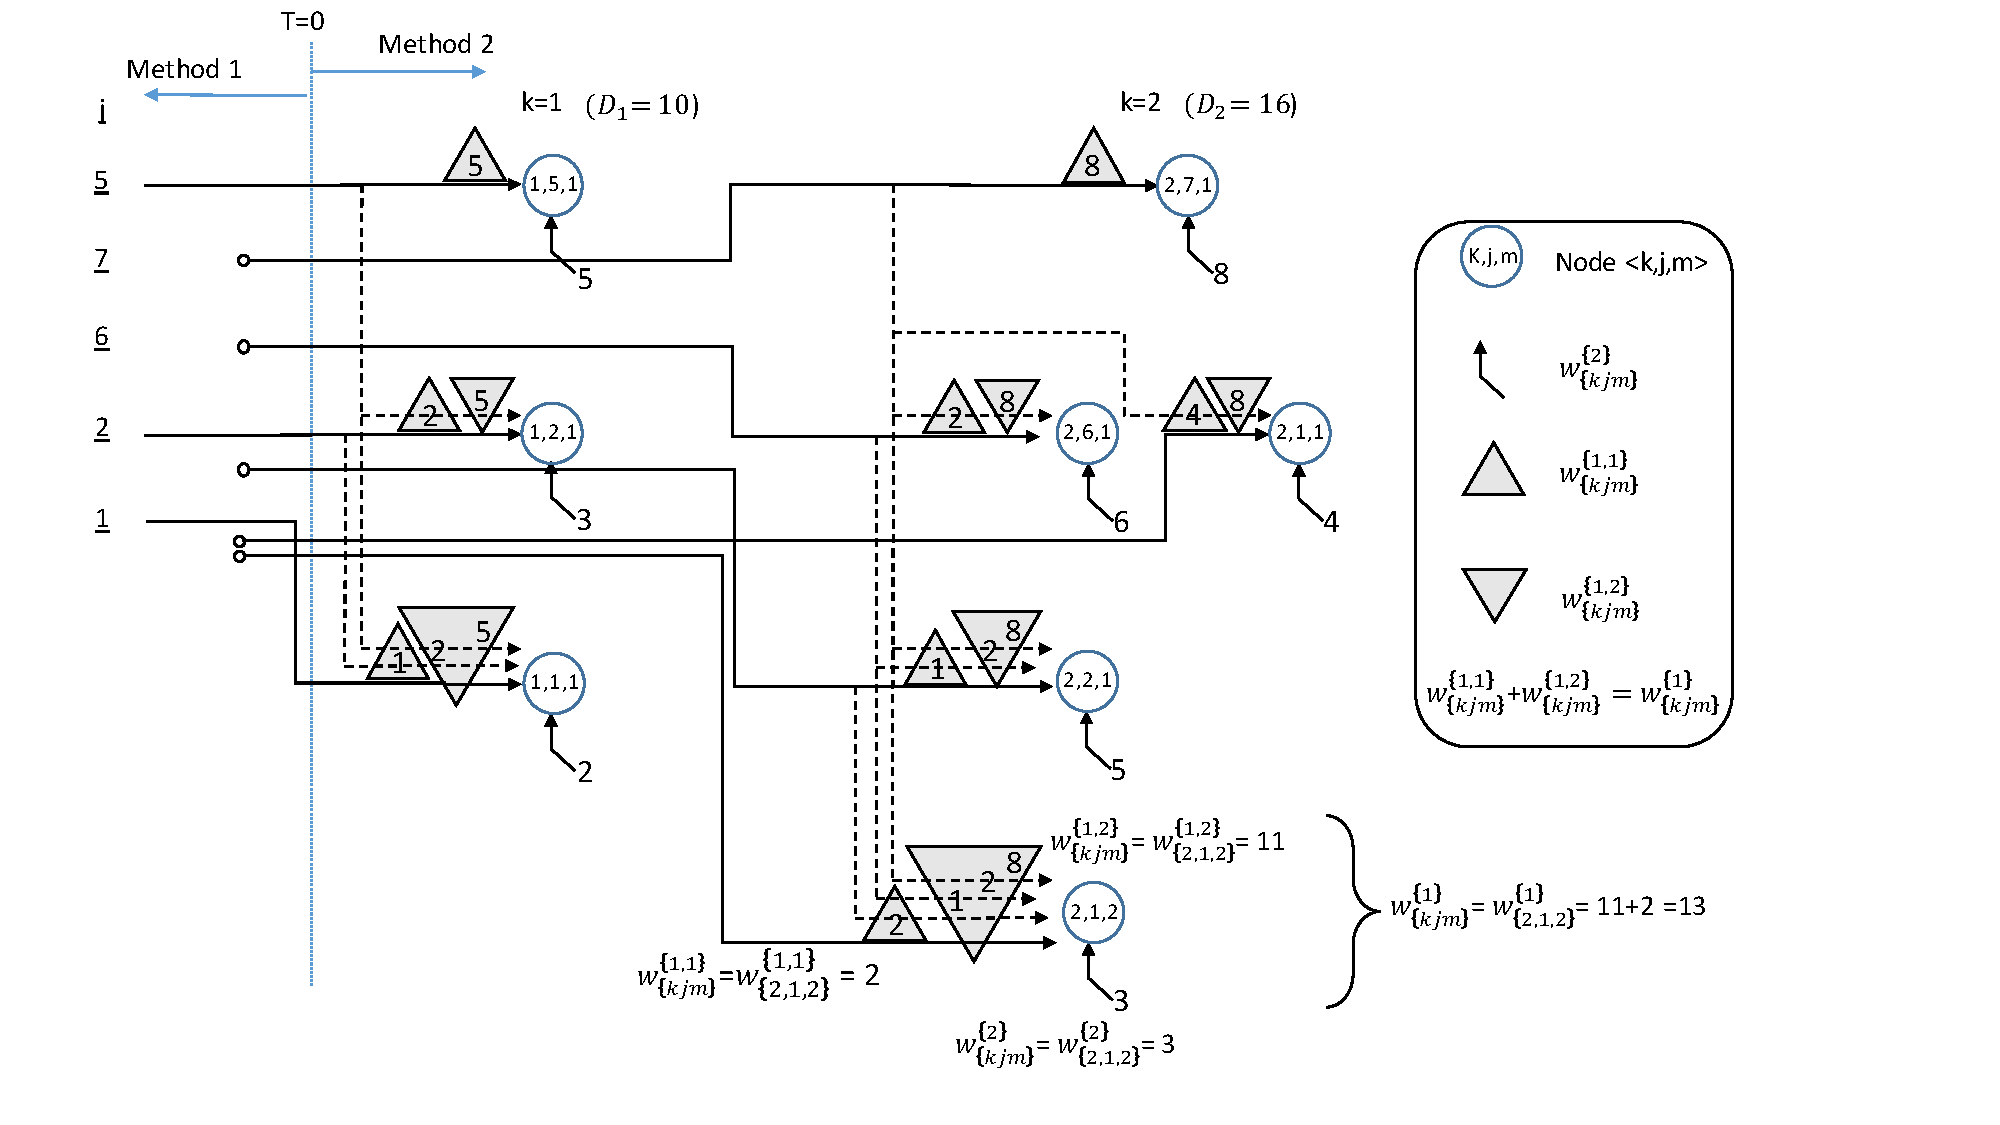
\includegraphics[trim={0 1cm 4cm 0},clip,width=\linewidth]{Example1_illustration.pdf}
\caption{Partial solution to Example 1}
\label{fig:example1_illustration}
\end{figure}
\FloatBarrier
%[sanchit] Give a broef explananation to the above and also attach the graphics for the example where these quantities have a value (see the sheet attachede for Example 1)
First, we present an MIP model for the case when the product demands are deterministic. It is represented as model ATO-CS-hybrid-D.\\
\textbf{Model ATO-CS-hybrid-D:}
\begin{alignat}{4}
& \text{Minimize: } \qquad \sum_{j \in J} f_{j}^{1} + \sum_{k \in K} \sum_{j \in J_k} f_{kj}^{2} \label{eq:fullmodelobj} \\
& w_{k,r_k,1}^{1,1} + w_{k,r_k,1}^{2} &&  = D_k , && \quad \forall k \in K \label{eq:c1} \\
& w_{klm}^{1,1} + w_{klm}^{2} &&  = w_{kjm}^{2} , && \quad \forall {<}k,j,m{>} \in N, \forall {<}k,l,m{>} \in R_{kjm} \label{eq:c2} \\
& w_{klm}^{1,2} &&  = w_{kjm}^{1} , && \quad \forall {<}k,j,m{>} \in N, \forall {<}k,l,m{>} \in R_{kjm} \label{eq:c3} \\
& w_{kjm}^{1,1} + w_{kjm}^{1,2} &&  = w_{kjm}^{1} , && \quad \forall {<}k,j,m{>} \in N \label{eq:c4} \\
& \sum_{k \in K_j} \sum_{m=1}^{\bar{m}_{kj}} w_{kjm}^{1} &&  = w_{j}^{1} , && \quad \forall j \in J \label{eq:c5} \\
& \sum_{m=1}^{\bar{m}_{kj}} w_{kjm}^{2} &&  = w_{kj}^{2} , && \quad \forall k \in K, j \in J_k \label{eq:c6} \\
& f_{j}^{1} &&  = b_j w_{j}^{1} + a_j \delta_{j}^{1}, && \quad \forall j \in J \label{eq:c7} \\
& w_{j}^{1} &&  \leq \bar{M}_{j} \delta_{j}^{1}, && \quad \forall j \in J \label{eq:c8} \\
& f_{kj}^{2} &&  = b_j w_{kj}^{2} + a_j \delta_{kj}^{2}, && \quad \forall k \in K, j \in J_k \label{eq:c9} \\
& w_{kj}^{2} &&  \leq \bar{M}_{kj} \delta_{kj}^{2}, && \quad \forall k \in K, j \in J_k \label{eq:c10} \\
& w_{kjm}^{1},w_{kjm}^{2},w_{kjm}^{1,1},w_{kjm}^{1,2},w_{j}^{1},w_{kj}^{2} && \in \mathbb{Z}^{+}, && \quad \forall j \in J, \forall k \in K_j, \forall m=1,\ldots \bar{m}_{kj} \label{eq:cdomain1} \\
& \delta_{j}^1, \delta_{kj}^2 && \in \mathbb{B}, && \quad \forall j \in J, \forall k \in K_j \label{eq:cdomain2} 
\end{alignat}
\\
Constraints \ref{eq:c1} relate the demand for each product, $k$, to the units of corresponding sub-assembly, $r_k$, being either procured directly from inventory ($w_{k,r_k,1}^{1,1}$) or assembled during Stage 2 ($w_{k,r_k,1}^{2}$). Constraints \ref{eq:c2} provide that for $w_{k,j,m}^{2}$ units of sub-assembly $j$, that are assembled during Stage 2, the equivalent units of its constituent sub-assembly, $l$ (where $n_{klm}$ is immediate child of $n_{kjm}$) are available either procured directly from inventory ($w_{k,l,m}^{1,1}$) or assembled during Stage 2 ($w_{k,l,m}^{2}$). Constraints \ref{eq:c3} enforce the relationship between the number of sub-assembly, $l$, that are used in the assembly of other sub-assemblies, $l^{'}$ (such that $n_{klm}$ is a child of $n_{kl^{'}m}$, directly or indirectly) during Stage 1, by recursively equating $w_{klm}^{1,2}$ to $w_{kjm}^{1}$ (where $n_{klm}$ is the immediate child of $n_{kjm}$). Note that $w_{klm}^{1,2}$ is not procured from inventory for assembly during Stage 2. Constraints \ref{eq:c4} provide total number of units of sub-assembly $j$ (in context of $n_{kjm}$), $w_{kjm}^{1}$, that are to be produced as per Method 1. Note that during Stage 1 (Method 1), assembly is done sub-assembly wise and not specific to each individual node $n_{kjm}$. As such, we sum over all such nodes corresponding to sub-assembly $j$ and get $w_{j}^{1}$ (constraints \ref{eq:c5}), the quantity that is produced contiguously during Stage 1. Constraints \ref{eq:c6} calculate $w_{kj}$, the quantity that is produced contiguously during Stage 2, for each sub-assembly $j$ specific to product $k$ of which it is part of BOM. Constraints \ref{eq:c7} and \ref{eq:c8} relates the cost of assembly of sub-assembly $j$ during Stage 1. Similarly, constraints \ref{eq:c9} and \ref{eq:c10} relates the cost of assembly of sub-assembly $j$ specific to product $k$ during Stage 2. The objective function combines the cost of production during Stage 1 and Stage 2 over all sub-assemblies and products.

For the case when the product demands are stochastic, the ATO-CS-hybrid methodology is implemented using a two-stage stochastic programming model with recourse. The demands of each product is modeled as a set of demand scenarios with some probability of occurrence. We need the following additional notation for the case of stochastic demands.
\begin{align*}
\begin{matrix}
s & \parbox[t]{0.8\textwidth}{Index of demand scenarios ($s=1,2,\ldots S$).} \\
p_s & \parbox[t]{0.8\textwidth}{Probability of occurance of scenario $s$.} \\
D_{ks} & \parbox[t]{0.8\textwidth}{Demand of product $k$ under scenario $s$.} \\
h & \parbox[t]{0.8\textwidth}{Inventory holding cost (or loss) per unit of any sub-assembly that is not used to meet products' demand.}
\end{matrix}
\end{align*}
Stage 1 decision variables:
\begin{align*}
w_{j}^{1}, f_{j}^{1} & = \parbox[t]{0.8\textwidth}{Number of $j^{th}$ sub-assembly to be produced by Method 1, and the associated cost, respectively.} \\
\delta_{j}^{1} &=
\begin{cases}
1, \parbox[t]{\textwidth}{if $w_{j}^{1}>0$,}\\
0, \parbox[t]{\textwidth}{otherwise.}
\end{cases}
\end{align*}
Stage 2 decision variables:
\begin{align*}
w_{kjs}^{2}, f_{kjs}^{2} & = \parbox[t]{0.8\textwidth}{Number of $j^{th}$ sub-assembly to be produced by Method 2 for product $k$, and the associated cost, respectively, under scenario $s$.} \\
\delta_{kjs}^{2} &=
\begin{cases}
1, \parbox[t]{\textwidth}{if $w_{kjs}^{2}>0$,}\\
0, \parbox[t]{0\textwidth}{otherwise.}
\end{cases}
\end{align*}
\setlength{\abovedisplayskip}{-6 pt}
\begin{align*}
& \begin{rcases}
w_{kjms}^{1}, w_{kjms}^{2} \\
w_{kjms}^{1,1}, w_{kjms}^{1,2}
\end{rcases} = \parbox[t]{0.8\textwidth}{The variables hold the same meaning in the context of $n_{kjm}$ as in the deterministic case, except with an additional index for each scenario $s$.} \\
& u_{js} = \parbox[t]{0.8\textwidth}{Number of $j^{th}$ sub-assembly that do not get utilized, under scenario $s$.}
\end{align*}
%
We now present model, ATO-CS-hybrid-S, where `S' stands for the stochastic version of the proposed methodology. \\ 
\textbf{Model ATO-CS-hybrid-S:}
%Method 1 of presenting (grouping by Stage 1 and Stage 2 separately)
\begin{alignat}{4}
& \text{Minimize: } \qquad && \sum_{j \in J} f_{j}^{1} \qquad + && \sum_{s=1}^{S} \left( \sum_{k \in K} \sum_{j \in J_k} f_{kjs}^{2} + \sum_{j\in J} h \, u_{js} \right) \label{eq:fullmodelobj_stochastic} \\
& f_{j}^{1} &&  = b_j w_{j}^{1} + a_j \delta_{j}^1, &&  \forall j \in J \label{eq:c7_stochastic} \\
& w_{j}^{1} &&  \leq \bar{M}_{j} \delta_{j}^1, &&  \forall j \in J \label{eq:c8_stochastic} \\
& \sum_{k \in K_j} \sum_{m=1}^{\bar{m}_{kj}} w_{kjms}^{1} + u_{js} &&  = w_{j}^{1} , &&  \forall j \in J, s=1,2,\ldots S \label{eq:c5_stochastic} \\
& w_{k,r_k,1,s}^{1,1} + w_{k,r_k,1,s}^{2} &&  \geq D_{k,s} , &&  \forall k \in K, s=1,2,\ldots S \label{eq:c1_stochastic} \\
& w_{klms}^{1,1} + w_{klms}^{2} &&  = w_{kjms}^{2} , &&  \forall {<}k,j,m{>} \in N, \forall {<}k,l,m{>} \in R_{kjm}, s=1,2,\ldots S \label{eq:c2_stochastic} \\
& w_{klms}^{1,2} &&  = w_{kjms}^{1} , &&  \forall {<}k,j,m{>} \in N, \forall {<}k,l,m{>} \in R_{kjm}, s=1,2,\ldots S \label{eq:c3_stochastic} \\
& w_{kjms}^{1,1} + w_{kjms}^{1,2} &&  = w_{kjms}^{1} , &&  \forall {<}k,j,m{>} \in N, s=1,2,\ldots S \label{eq:c4_stochastic} \\
& \sum_{m=1}^{\bar{m}_{kj}} w_{kjms}^{2} &&  = w_{kjs}^{2} , &&  \forall k \in K, j \in J_k, s=1,2,\ldots S \label{eq:c6_stochastic} \\
& f_{kjs}^{2} &&  = b_j w_{kjs}^{2} + a_j \delta_{kjs}^2, &&  \forall k \in K, j \in J_k, s=1,2,\ldots S \label{eq:c9_stochastic} \\
& w_{kjs}^{2} &&  \leq \bar{M}_{kj} \delta_{kjs}^{2}, &&  \forall k \in K, j \in J_k, s=1,2,\ldots S \label{eq:c10_stochastic} \\
& \begin{rcases}
w_{j}^{1},u_{js},w_{kjs}^{2},w_{kjms}^{1}, \\
w_{kjms}^{1,1},w_{kjms}^{1,2},w_{kjms}^{2} 
\end{rcases}
&& \in \mathbb{Z}^{+}, &&  \forall j \in J, \forall k \in K_j, \forall m=1,\ldots \bar{m}_{kj}, \forall s=1,2,\ldots S \label{eq:cdomain1_stochastic} \\
& \delta_{j}^1, \delta_{kjs}^2 && \in \mathbb{B}, &&  \forall j \in J, \forall k \in K_j,\forall s=1,2,\ldots S \label{eq:cdomain2_stochastic} 
\end{alignat}
%%Method 2 of presenting (more like deterministic case)
%\begin{alignat}{4}
%& \text{Minimize: } \qquad && \sum_{j \in J} f_{j}^{1} \qquad + && \sum_{s=1}^{S} \left( \sum_{k \in K} \sum_{j \in J_k} f_{kjs}^{2} + \sum_{j\in J} h \, u_{js} \right) \label{eq:fullmodelobj_stochastic} \\
%& w_{k,r_k,1,s}^{1,1} + w_{k,r_k,1,s}^{2} &&  \geq D_{k,s} , &&  \forall k \in K, s=1,2,\ldots S \label{eq:c1_stochastic} \\
%& w_{klms}^{1,1} + w_{klms}^{2} &&  = w_{kjms}^{2} , &&  \forall {<}k,j,m{>} \in N, \forall {<}k,l,m{>} \in R_{kjm}, s=1,2,\ldots S \label{eq:c2_stochastic} \\
%& w_{klms}^{1,2} &&  = w_{kjms}^{1} , &&  \forall {<}k,j,m{>} \in N, \forall {<}k,l,m{>} \in R_{kjm}, s=1,2,\ldots S \label{eq:c3_stochastic} \\
%& w_{kjms}^{1,1} + w_{kjms}^{1,2} &&  = w_{kjms}^{1} , &&  \forall {<}k,j,m{>} \in N, s=1,2,\ldots S \label{eq:c4_stochastic} \\
%& \sum_{k \in K_j} \sum_{m=1}^{\bar{m}_{kj}} w_{kjms}^{1} &&  = w_{j}^{1} , &&  \forall j \in J \label{eq:c5_stochastic} \\
%& \sum_{m=1}^{\bar{m}_{kj}} w_{kjms}^{2} &&  = w_{kjs}^{2} , &&  \forall k \in K, j \in J_k, s=1,2,\ldots S \label{eq:c6_stochastic} \\
%& f_{j}^{1} &&  = u_j w_{j}^{1} + s_j \delta_{j}^1, &&  \forall j \in J \label{eq:c7_stochastic} \\
%& w_{j}^{1} &&  \leq \bar{M}_{j} \delta_{j}^1, &&  \forall j \in J \label{eq:c8_stochastic} \\
%& f_{kjs}^{2} &&  = u_j w_{kjs}^{2} + s_j \delta_{kjs}^2, &&  \forall k \in K, j \in J_k, s=1,2,\ldots S \label{eq:c9_stochastic} \\
%& w_{kjs}^{2} &&  \leq \bar{M}_{kj} \delta_{kjs}^{2}, &&  \forall k \in K, j \in J_k, s=1,2,\ldots S \label{eq:c10_stochastic} \\
%& \begin{rcases}
%w_{j}^{1},u_{ks},w_{kjs}^{2},w_{kjms}^{1}, \\
%w_{kjms}^{1,1},w_{kjms}^{1,2},w_{kjms}^{2} 
%\end{rcases}
%&& \in \mathbb{Z}^{+}, &&  \forall j \in J, \forall k \in K_j, \forall m=1,\ldots \bar{m}_{kj}, \forall s=1,2,\ldots S \label{eq:cdomain1_stochastic} \\
%& \delta_{j}^1, \delta_{kjs}^2 && \in \mathbb{B}, &&  \forall j \in J, \forall k \in K_j,\forall s=1,2,\ldots S \label{eq:cdomain2_stochastic} 
%\end{alignat}

\section{A Numerical Example \label{sec:numerical_example}}
\begin{example}
\label{ex:1}
We present a small example consisting of 2 products and 7 sub-assemblies for an assembly job shop configuration in the presence of commonality of sub-assemblies across products (as is evident in the BOM of the products shown in Figure \ref{fig:normal_bom_prods}). The data for this example is provided in Table \ref{table:products_data} and Table \ref{table:subassemblies_composition}. Figure \ref{fig:kjm_bom_prods} illustrates the BOMs of the products using a tree graph, wherein each node has a unique label of the form ${<}k,j,m{>}$, where $k$ and $j$ are indices for the product and sub-assembly, respectively, and $m$ is the multiplicity index of the sub-assembly in that product.

Through this example, we will show the superiority of ATO-CS-hybrid over other methodologies for both the cases when demands are deterministic and stochastic.

%
%Figure:BOM products
\begin{figure}[htbp]
\centering
\begin{subfigure}{0.6\textwidth}
\centering
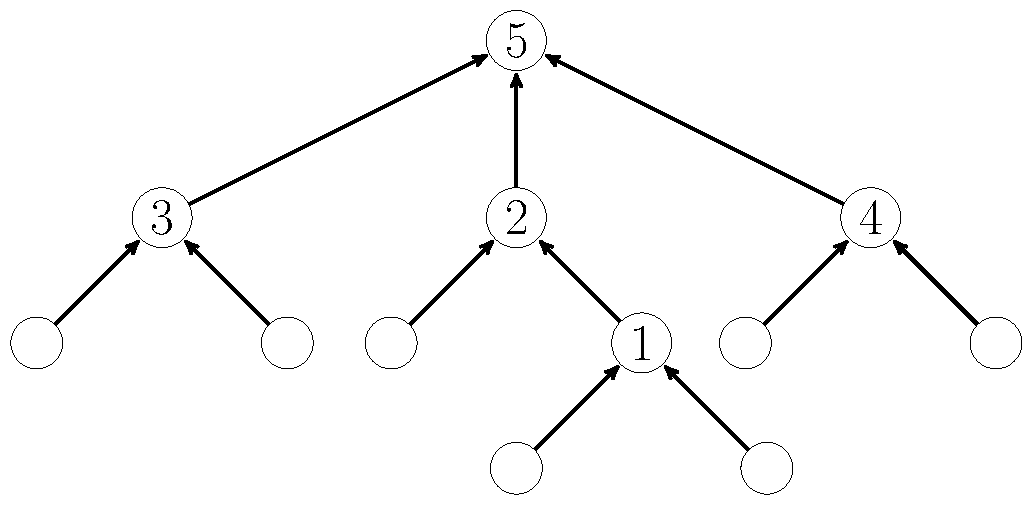
\includegraphics[width=\linewidth]{figure_prod1_bom.pdf}
\caption{Product 1}
\label{fig:bom_prod1}
\end{subfigure}%
\begin{subfigure}{0.4\textwidth}
\centering
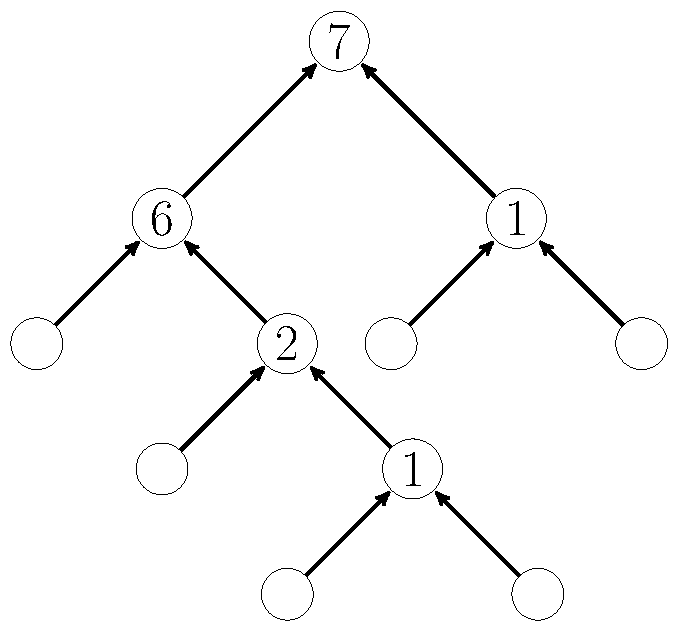
\includegraphics[width=\linewidth]{figure_prod2_bom.pdf}
\caption{Product 2}
\label{fig:bom_prod2}
\end{subfigure} 
\caption{Example \ref{ex:1}-BOM of products}
\label{fig:normal_bom_prods}
\end{figure}
%
\begin{table}[htbp]
\centering
\caption{Products Data}
\label{table:products_data}
\begin{tabular}{|c|c|c|}
\hline
Product ($k$) & Root sub-assembly ($r_k$) \\ \hline
1 & 5 \\
2 & 7 \\
\hline
\end{tabular}
\end{table}

%
\begin{table}[htbp]
\centering
\caption{Composition of sub-assemblies}
\label{table:subassemblies_composition}
\begin{tabular}{|c|c|c|c|}
\hline
Sub-assembly ($j$) & Set of children ($R_j$) & Setup cost ($a_j$) & Unit assembly cost ($b_j$) \\ \hline
1 & $\phi$ & 10 & 1 \\
2 & \{1\} & 10 & 1 \\
3 & $\phi$ & 5 & 1 \\
4 & $\phi$ & 5 & 1 \\
5 & \{2,3,4\} & 5 & 2 \\
6 & \{2\} & 5 & 1 \\ 
7 & \{1,6\} & 5 & 1 \\ 
\hline
\end{tabular}
\end{table}

%Figure:kjm representation products
\begin{figure}[htbp]
\centering
\begin{subfigure}{0.6\textwidth}
\centering
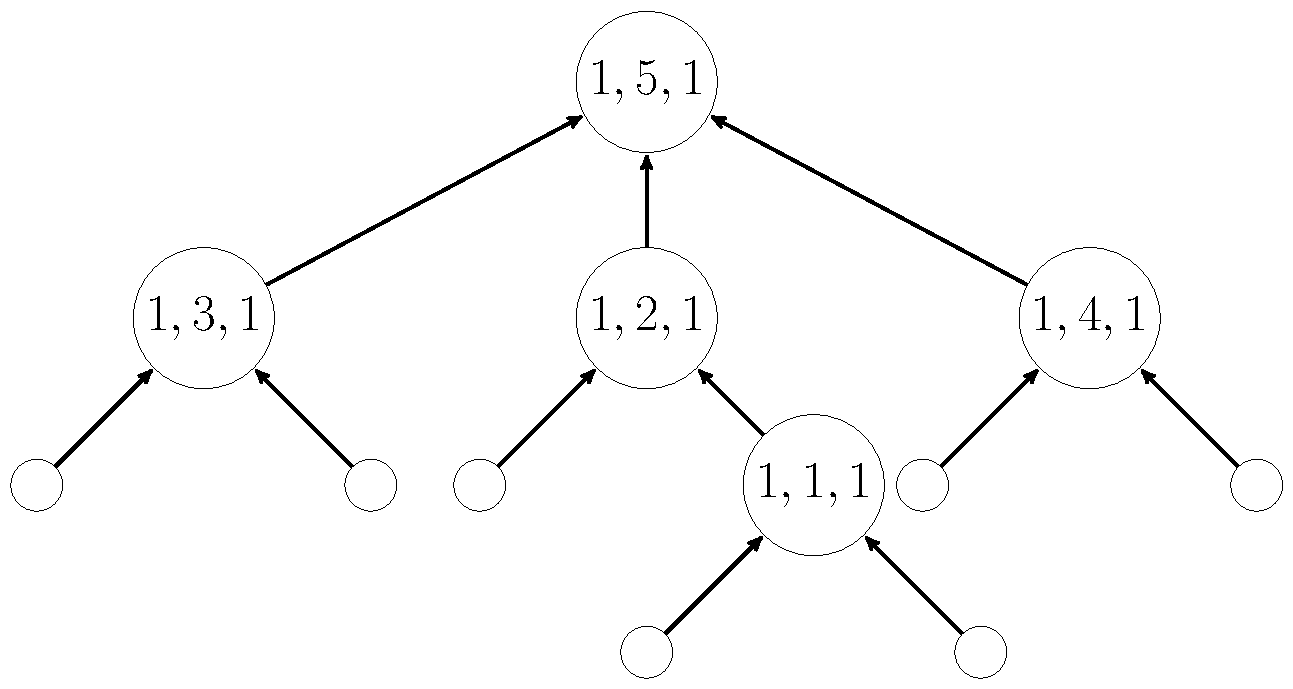
\includegraphics[width=\linewidth]{figure_prod1_graph_kjm.pdf}
\caption{Product 1}
\label{fig:kjm_bom_prod1}
\end{subfigure}%
\begin{subfigure}{0.4\textwidth}
\centering
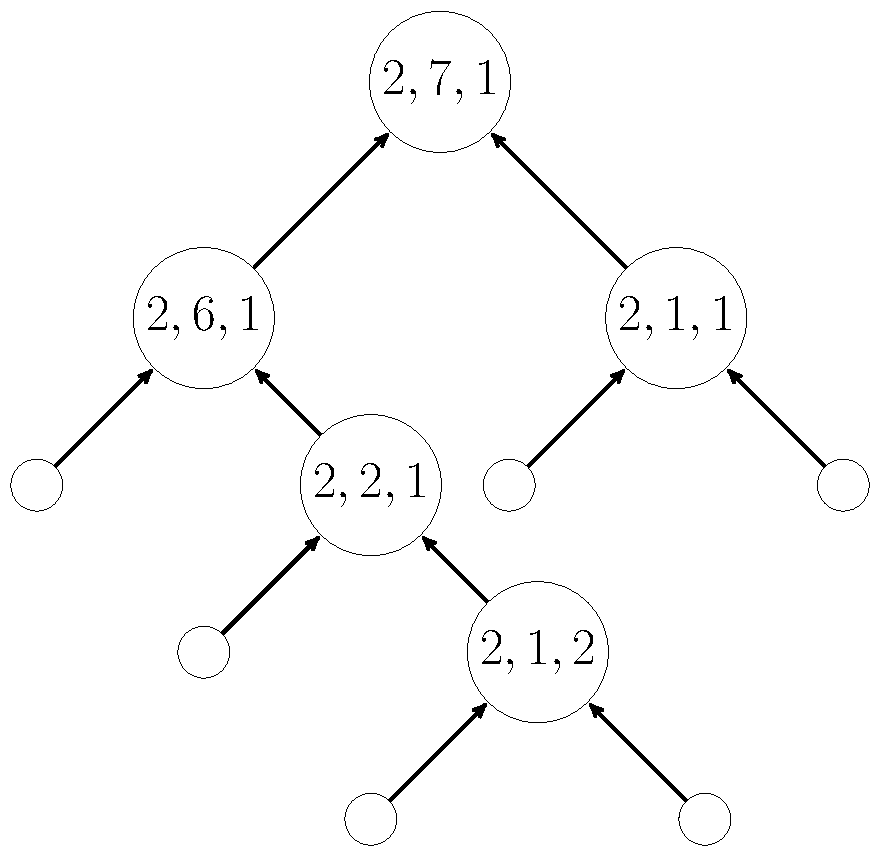
\includegraphics[width=\linewidth]{figure_prod2_graph_kjm.pdf}
\caption{Product 2}
\label{fig:kjm_bom_prod2}
\end{subfigure} 
\caption{Example \ref{ex:1}-Unique representation of each sub-assembly (node) in BOM of products}
\label{fig:kjm_bom_prods}
\end{figure}
\end{example}
\FloatBarrier
\noindent
\textbf{SOLUTION:} \\
\textbf{Deterministic demand.}
We present the cost of production by three methodologies, namely Method 1 (Table \ref{table:cost_MTS}), Method 2 (Table \ref{table:cost_MTO}) and ATO-CS-hybrid (Table \ref{table:cost_ATO-CS-hybrid}) when the demand for the products is $D_1=10$ and $D_2=10$.

\begin{table}[htbp]
\caption{Example 1: Cost of production by Method 1 (sub-assembly-specific) for deterministic demand ($D_1=10, D_2=10$)}
\begin{center}
\begin{tabular}{|c|r|}
\hline
Sub-assembly (quantity) & Cost \\ \hline
1 (30) & 10+1x30=40 \\ \hline
3 (10) & 5+1x10=15 \\ \hline
4 (10) & 5+1x10=15 \\ \hline
2 (20) & 10+1x20=30 \\ \hline
6 (10) & 5+1x10=15 \\ \hline
7 (10) & 5+1x10=15 \\ \hline
5 (10) & 5+2x10=25 \\ \hline
Total cost: & 155 \\ \hline
\end{tabular}
\end{center}
\label{table:cost_MTS}
\end{table}

\begin{table}[htbp]
\centering
\caption{Example 1-Cost of production by Method 2 (product-specific) for deterministic demand ($D_1=10, D_2=10$)}
\begin{tabular}{|c|c|r|}
\hline
Product & Sub-assembly (quantity) & Cost \\ \hline
\multicolumn{ 1}{|c|}{1 } & 1 (10) & 10+1x10=20 \\ \cline{ 2- 3}
\multicolumn{ 1}{|l|}{} & 3 (10) & 5+1x10=15 \\ \cline{ 2- 3}
\multicolumn{ 1}{|l|}{} & 4 (10) & 5+1x10=15 \\ \cline{ 2- 3}
\multicolumn{ 1}{|l|}{} & 2 (10) & 10+1x10=20 \\ \cline{ 2- 3}
\multicolumn{ 1}{|l|}{} & 5 (10) & 5+2x10=25 \\ \hline
\multicolumn{ 1}{|c|}{2} & 1 (20) & 10+1x20=30 \\ \cline{ 2- 3}
\multicolumn{ 1}{|l|}{} & 2 (10) & 10+1x10=20 \\ \cline{ 2- 3}
\multicolumn{ 1}{|l|}{} & 6 (10) & 5+1x10=15 \\ \cline{ 2- 3}
\multicolumn{ 1}{|l|}{} & 7 (10) & 5+1x10=15 \\ \hline
\multicolumn{ 2}{|r|}{Total cost:} & \multicolumn{1}{r|}{175} \\ \hline
\end{tabular}
\label{table:cost_MTO}
\end{table}
\FloatBarrier

As expected, cost of production by Method 1 is smaller than that by Method 2 since all units of a sub-assembly are assembled together thus reducing cost by economy of scale.

\begin{table}[htbp]
\caption{Example 1: Cost of production by ATO-CS-hybrid for deterministic demand ($D_1=10, D_2=10$)}
\label{table:cost_ATO-CS-hybrid}
\begin{center}
\begin{tabular}{|c|c|c|}
\hline
\multirow{3}{*}{Sub-assembly} & \multirow{3}{6cm}{Quantity produced by \\Method 1 (cost) $\equiv w_{j}^{1} (f_{j}^{1})$} & \multirow{3}{6cm}{Quantity produced by Method 2, $w_{kj}^{2}$, specific to product, $k$ and its cost, $f_{kj}^{2} \equiv k, w_{kj}^{2} (f_{kj}^{2})$}  \\
 & & \\
 & & \\ \hline
1 & 30 (40) & $\phi$, 0 (0) \\ \hline
3 & 0 (0) & 1, 10 (15) \\ \hline
4 & 0 (0) & 1, 10 (15) \\ \hline
2 & 20 (30) & $\phi$, 0 (0) \\ \hline
6 & 0 (0) & 2, 10 (15) \\ \hline
7 & 0 (0) & 2, 10 (15) \\ \hline
5 & 0 (0) & 1, 10 (25) \\ \hline
\multirow{2}{*}{Total cost:} & 70 & 85 \\ \cline{2-3}
 & \multicolumn{2}{c|}{155} \\ \hline
\end{tabular}
\end{center}
\end{table}
\FloatBarrier

Model ATO-CS-hybrid-D is solved for the data given in this example, and it can be seen from the solution presented in Table \ref{table:cost_ATO-CS-hybrid} that it differs from Method 1 solution only in that it operates in a two-stage manner rather than a single-stage production, but otherwise, just like Method 1, all units of a single sub-assembly are assembled together. \\

\textbf{Stochastic demand.} 
We present the cost of production by four methodologies, namely MTS (Table \ref{table:cost_MTS_stochastic}), MTO (Table \ref{table:cost_MTO_stochastic}), ATO (Table \ref{table:cost_ATO_stochastic}) and ATO-CS-hybrid (Table \ref{table:cost_ATO-CS-hybrid_stochastic}) when the demands for products follow uniform distributions. Let $D_1 \sim \text{Unif}(9,11)$ and $D_2 \sim \text{Unif}(9,11)$. As such, there are nine scenarios of products' demand. For a fair comparison among different methodologies, it is assumed that full demand for both the products has to be met under all scenarios. Under this premise, it is understood that the appropriate amount of sub-assemblies be assembled and stocked up as inventory prior to actual demand realization. \\ 

\begin{table}[htbp]
\caption{Example 1: Cost of production and inventory losses in MTS system for stochastic demand ($D_1 \sim \text{Unif}(9,11), D_2 \sim \text{Unif}(9,11)$)}
\label{table:cost_MTS_stochastic}
\begin{center}
\resizebox{\textwidth}{!}{
\begin{tabular}{|c|c|c|c|c|c|c|c|c|c|c|}
\hline
\multirow{2}{*}{Sub-assembly} & \multirow{2}{4cm}{Quantity produced \\by Method 1 (cost)} & \multicolumn{9}{c|}{Scenarios represented by $(D_1,D_2)$} \\ \cline{3-11}
& & (9,9) & (9,10) & (9,11) & (10,9) & (10,10) & (10,11) & (11,9) & (11,10) & (11,11) \\ \hline
\multicolumn{2}{|c|}{} & \multicolumn{9}{c|}{Inventory cost of sub-assemblies unused} \\ \hline
1 & 33 (43) & 6h & 4h & 2h & 5h & 3h & 1h & 4h & 2h & 0 \\ \hline
3 & 11 (16) & 2h & 2h & 2h & 1h & 1h & 1h & 0  & 0  & 0 \\ \hline
4 & 11 (16) & 2h & 2h & 2h & 1h & 1h & 1h & 0  & 0  & 0 \\ \hline
2 & 22 (32) & 4h & 3h & 2h & 3h & 2h & 1h & 2h & 1h & 0 \\ \hline
6 & 11 (16) & 2h & 1h & 0  & 2h & 1h & 0  & 2h & 1h & 0 \\ \hline
7 & 11 (16) & 2h & 1h & 0  & 2h & 1h & 0  & 2h & 1h & 0 \\ \hline
5 & 11 (27) & 2h & 2h & 2h & 1h & 1h & 1h & 0  & 0  & 0 \\ \hline
Total cost: & 166 & 20h & 15h & 10h & 15h & 10h & 5h & 10h & 5h & 0 \\ \hline
Expected cost: & \multicolumn{10}{c|}{166+1/9$\times$90h=166+10h} \\ \hline
\end{tabular}
}
\end{center}
\end{table}
\FloatBarrier

\begin{table}[htbp]
\caption{Example 1: Cost of production and inventory losses in MTO system for stochastic demand ($D_1 \sim \text{Unif}(9,11), D_2 \sim \text{Unif}(9,11)$)}
\label{table:cost_MTO_stochastic}
\begin{center}
\resizebox{\textwidth}{!}{
\begin{tabular}{|c|c|c|c|c|c|c|c|c|c|c|}
\hline
\multirow{2}{*}{Product} & \multirow{2}{*}{Sub-assembly} & \multicolumn{9}{c|}{Scenarios represented by $(D_1,D_2)$} \\ \cline{3-11}
&  & (9,9) & (9,10) & (9,11) & (10,9) & (10,10) & (10,11) & (11,9) & (11,10) & (11,11) \\ \hline
\multicolumn{2}{|c|}{} & \multicolumn{9}{c|}{Quantity produced by Method 2 (cost)} \\ \hline
\multirow{5}{*}{1} & 1 & 9 (19) & 9 (19) & 9 (19) & 10 (20) & 10 (20) & 10 (20) & 11 (21) & 11 (21) & 11 (21) \\ \cline{2-11}
 & 3 & 9 (14) & 9 (14) & 9 (14) & 10 (15) & 10 (15) & 10 (15) & 11 (16) & 11 (16) & 11 (16) \\ \cline{2-11} 
 & 4 & 9 (14) & 9 (14) & 9 (14) & 10 (15) & 10 (15) & 10 (15) & 11 (16) & 11 (16) & 11 (16) \\ \cline{2-11} 
 & 2 & 9 (19) & 9 (19) & 9 (19) & 10 (20) & 10 (20) & 10 (20) & 11 (21) & 11 (21) & 11 (21) \\ \cline{2-11}
 & 5 & 9 (23) & 9 (23) & 9 (23) & 10 (25) & 10 (25) & 10 (25) & 11 (27) & 11 (27) & 11 (27) \\ \hline
\multirow{4}{*}{2} & 1 & 18 (28) & 20 (30) & 22 (32) & 18 (28) & 20 (30) & 22 (32) & 18 (28) & 20 (30) & 22 (32) \\ \cline{2-11}
 & 2 & 9 (19) & 10 (20) & 11 (21) & 9 (19) & 10 (20) & 11 (21) & 9 (19) & 10 (20) & 11 (21) \\ \cline{2-11}
 & 6 & 9 (14) & 10 (15) & 11 (16) & 9 (14) & 10 (15) & 11 (16) & 9 (14) & 10 (15) & 11 (16) \\ \cline{2-11}
 & 7 & 9 (14) & 10 (15) & 11 (16) & 9 (14) & 10 (15) & 11 (16) & 9 (14) & 10 (15) & 11 (16) \\ \hline
\multicolumn{2}{|r|}{Total cost:} & 164 & 169 & 174 & 170 & 175 & 180 & 176 & 181 & 186 \\ \hline
\multicolumn{2}{|r|}{Expected cost:} & \multicolumn{9}{c|}{1/9$\times$1575=175} \\ \hline
\end{tabular}
}
\end{center}
\end{table}
\FloatBarrier

For MTS, we have to stock the sub-assemblies anticipating the worst-case scenario, since the methodology doesn't allow the sub-assemblies to be assembled post demand realization. Column 2 of Table \ref{table:cost_MTS_stochastic} shows the quantity of sub-assemblies assembled before demand realization. Columns 3-11 show the cost of inventory for the sub-assemblies left unused after demand realization. Under the assumption that all sub-assemblies be stocked up for the worst-case scenario, MTS is expected to deliver the least lead times (theoretically zero) for products if the timing aspect of the scheduling is also considered. But, this advantage is countered by higher expected cost through inventory losses.

For MTO, all the sub-assemblies are started for assembly only after the products' demands are realized. All  the sub-assemblies specific to a product are assembled first before starting with the next product. The cost of production is given in Columns 3-11 of Table \ref{table:cost_MTO_stochastic}. Note that MTO does not result into inventory losses, since everything is made post demand realization. When the inventory holding costs or losses are significant, MTO is expected to perform the best in terms of production and inventory costs. This gain is offset by large expected lead times for products, if the timing aspect of the scheduling is also considered.

\begin{table}[htbp]
\caption{Example 1: Cost of production and inventory losses in ATO system for stochastic demand ($D_1 \sim \text{Unif}(9,11), D_2 \sim \text{Unif}(9,11)$)}
\label{table:cost_ATO_stochastic}
\begin{center}
\resizebox{\textwidth}{!}{
\begin{tabular}{|c|c|c|c|c|c|c|c|c|c|c|}
\hline
\multirow{2}{*}{Sub-assembly} & \multirow{2}{4cm}{Quantity produced \\by Method 1 (cost)} & \multicolumn{9}{c|}{Scenarios represented by $(D_1,D_2)$} \\ \cline{3-11}
&  & (9,9) & (9,10) & (9,11) & (10,9) & (10,10) & (10,11) & (11,9) & (11,10) & (11,11) \\ \hline
\multicolumn{2}{|c|}{} & \multicolumn{9}{c|}{Inventory cost of sub-assemblies unused} \\ \hline
1 & 33 (43) & 6h & 4h & 2h & 5h & 3h & 1h & 4h & 2h & 0 \\ \hline
3 & 11 (16) & 2h & 2h & 2h & 1h & 1h & 1h & 0  & 0  & 0 \\ \hline
4 & 11 (16) & 2h & 2h & 2h & 1h & 1h & 1h & 0  & 0  & 0 \\ \hline
2 & 22 (32) & 4h & 3h & 2h & 3h & 2h & 1h & 2h & 1h & 0 \\ \hline
6 & 11 (16) & 2h & 1h & 0  & 2h & 1h & 0  & 2h & 1h & 0 \\ \hline
\multicolumn{2}{|c|}{} & \multicolumn{9}{c|}{Quantity produced by Method 2 (cost)} \\ \hline
7 & 0 (0) & 9 (14) & 10 (15) & 11 (16) & 9 (14) & 10 (15) & 11 (16) & 9 (14) & 10 (15) & 11 (16) \\ \hline
5 & 0 (0) & 9 (23) & 9 (23) & 9 (23) & 10 (25) & 10 (25) & 10 (25) & 11 (27) & 11 (27) & 11 (27) \\ \hline
Total cost: & 123 & 37+16h & 38+12h & 39+8h & 39+12h & 40+8h & 41+4h & 41+8h & 42+4h & 43 \\ \hline
Expected cost: & \multicolumn{10}{c|}{123+1/9$\times$(360+72h)=163+8h} \\ \hline
\end{tabular}
}
\end{center}
\end{table}
\FloatBarrier

ATO is very similar to MTS, except that the final sub-assemblies (corresponding to products) are not assembled in advance. The rest of the sub-assemblies are assembled and stocked up expecting the worst-case scenario. Column 2 of Table \ref{table:cost_ATO_stochastic} shows the quantity of sub-assemblies assembled before demand realization. Columns 3-11 show the cost of inventory for the sub-assemblies left unused after demand realization for all the sub-assemblies except the ones corresponding to the products. Sub-assemblies $5$ and $7$ are assembled post demand realization for Products $1$ and $2$ respectively, and their production cost is given in Columns 3-11. 

\begin{table}[htbp]
\caption{Example 1: Cost of production and inventory losses in ATO-CS-hybrid system for stochastic demand ($D_1 \sim \text{Unif}(9,11), D_2 \sim \text{Unif}(9,11)$)}
\label{table:cost_ATO-CS-hybrid_stochastic}
\begin{center}
\resizebox{\textwidth}{!}{
\begin{tabular}{|c|c|c|c|c|c|c|c|c|c|c|c|}
\hline
\multicolumn{3}{|c|}{Production by Method 1} & \multicolumn{9}{c|}{Scenarios represented by $(D_1,D_2)$} \\ \hline
\multirow{2}{*}{Sub-assembly ($j$)} & \multirow{2}{*}{Quantity ($w_{j}^{1}$)} & \multirow{2}{*}{Cost ($f_{j}^{1}$)} & (9,9) & (9,10) & (9,11) & (10,9) & (10,10) & (10,11) & (11,9) & (11,10) & (11,11) \\ \cline{4-12}
& & & \multicolumn{9}{c|}{Inventory cost of sub-assemblies unused} \\ \hline
2 & 20 & 60 & 2h & h & 0 & 1 & 0 & 0 & 0 & 0 & 0 \\ \hline
\multicolumn{12}{|c|}{} \\ \hline
Product ($k$) & Sub-assembly (j) & Multiplicity ($m$) & \multicolumn{9}{c|}{Quantity produced by Method 2 (cost) $\equiv w_{kjm}^{2} (f_{kjm}^{2})$} \\ \hline
\multirow{5}{*}{1} & 1 & 1 & 0 (0) & 0 (0) & 0 (0) & 0 (0) & 0 (0) & 0 (0) & 0 (0) & 1 (11) & 1 (11) \\ \cline{2-12}
 & 3 & 1 & 9 (14) & 9 (14) & 9 (14) & 10 (15) & 10 (15) & 10 (15) & 11 (16) & 11 (16) & 11 (16) \\ \cline{2-12}
 & 4 & 1 & 9 (14) & 9 (14) & 9 (14) & 10 (15) & 10 (15) & 10 (15) & 11 (16) & 11 (16) & 11 (16) \\ \cline{2-12}
 & 2 & 1 & 0 (0) & 0 (0) & 0 (0) & 0 (0) & 0 (0) & 0 (0) & 0 (0) & 1 (11) & 1 (11) \\ \cline{2-12}
 & 5 & 1 & 9 (23) & 9 (23) & 9 (23) & 10 (25) & 10 (25) & 10 (25) & 11 (27) & 11 (27) & 11 (27) \\ \hline
\multirow{4}{*}{2} & \multirow{2}{*}{1} & 1 & 9 (19) & 10 (20) & 11 (21) & 9 (19) & 10 (20) & 11 (21) & 9 (19) & 10 (20) & 11 (21) \\
 & & 2 & 0 (0) & 0 (0) & 0 (0) & 0 (0) & 0 (0) & 1 (11)  & 0 (0) & 0 (0) & 1 (11) \\ \cline{2-12} 
 & 2 & 1 & 0 (0) & 0 (0) & 0 (0) & 0 (0) & 0 (0) & 1 (11)  & 0 (0) & 0 (0) & 1 (11) \\ \cline{2-12} 
 & 6 & 1 & 9 (14) & 10 (15) & 11 (16) & 9 (14) & 10 (15) & 11 (16) & 9 (14) & 10 (15) & 11 (16) \\ \cline{2-12}
 & 7 & 1 & 9 (14) & 10 (15) & 11 (16) & 9 (14) & 10 (15) & 11 (16) & 9 (14) & 10 (15) & 11 (16) \\ \hline
\multicolumn{2}{|r|}{Total cost:} & 60 & 98+2h & 101+h & 104 & 102+h & 106 & 130 & 105 & 131 & 156 \\ \hline
\multicolumn{2}{|r|}{Expected cost:} & \multicolumn{10}{c|}{60+1/9$\times$(1033+4h)=174.78+0.44h} \\ \hline
\end{tabular}
}
\end{center}
\end{table}
\FloatBarrier

The solution obtained for the ATO-CS-hybrid system is presented in Table \ref{table:cost_ATO-CS-hybrid_stochastic}. Even though the solution is not optimal to model ATO-CS-hybrid-S, the result characterizes the superiority of ATO-CS-hybrid methodology over others. Method 1 production takes place before demand realization and as such, $20$ units of sub-assembly $2$ are assembled in advance, and kept in inventory. For different scenarios, these units are diverted to be used in assembly of different products. For example, when the demand scenario $(10,9)$ is realized, i.e. Column $7$, we can effectively use $10$ units of this sub-assembly towards fulfillment of Product $1$ demand, and other $9$ towards Product $2$. A single unit of the sub-assembly goes un-utilized, and contributes towards inventory loss of $h$. Method 2 production takes place upon individual product demand realization, and as such when a scenario occurs, the remaining and least necessary sub-assemblies assembled specific to one product at-a-time. \\

We now present the results for all the four methodologies in Figure \ref{fig:comparison_all_4} for different values of $h$. Clearly, the cost incurred by ATO is lesser than that by MTS. ATO is better than ATO-CS-hybrid only marginally for small values of $h$, but is otherwise outperformed for higher values of $h$ by ATO-CS-hybrid. As for MTO, it results in least cost for higher values of $h$, even though ATO-CS-hybrid has only slightly higher cost. But this advantage of MTO is significantly offset if the timing aspect of scheduling is taken into account. As such, MTO would result into largest lead times for products.
%
%Figure:Comaprison among all 4 methodolgoies
\begin{figure}[htbp]
\centering
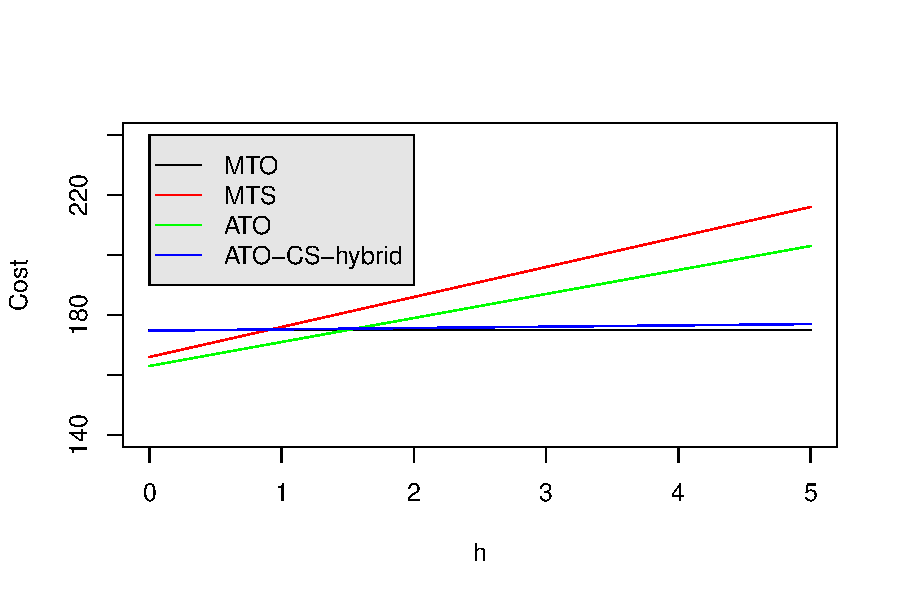
\includegraphics[width=0.8\linewidth]{comparsion_all_4.pdf}
\caption{Example 1: Comparison of expected cost (production and inventory loss) with MTO, MTS, ATO and ATO-CS-hybrid system}
\label{fig:comparison_all_4}
\end{figure}

\section{Conclusion \label{sec:conclusion}}

In this paper, we consider deterministic as well as stochastic demand scenarios for products which share certain sub-assemblies in their BOM. The production environment mimics an assembly job-shop, even though the timing aspect is not considered here. The objective is to minimize production cost and inventory loss. We propose a novel methodology, ATO-CS-hybrid, and formulate two integer programs, model ATO-CS-hybrid-D and model ATO-CS-hybrid-S, for the case when demands are deterministic and stochastic, respectively. Its performance is compared with three commonly practiced methodologies, MTO, MTS and ATO through a short example. The results show that ATO-CS-hybrid is superior to the other methodologies. The initial results are satisfactory, therefore we propose to do the following in future in order to explore the usefulness of ATO-CS-hybrid. (1) We propose to consider timing aspect of the jobs (products) as well, as would be the case in a full fledged assembly job-shop. (2) Model ATO-CS-hybrid is a two stage stochastic program and needs be solved to obtain optimal solution. We propose to implement an appropriate exact algorithm that will be able to handle even the large test data as we investigate the performance of ATO-CS-hybrid rigorously.

\bibliography{references}

\end{document}